\documentclass[journal,twocolumn]{IEEEtran}

\usepackage[utf8]{inputenc}
\usepackage[T1]{fontenc}
\usepackage{amsmath}
\usepackage{graphicx}
\usepackage{float}
\usepackage{booktabs}
\usepackage{cite}
\usepackage{url}
\usepackage{array}
\usepackage{siunitx}

\begin{document}

\title{Identification and Control of a Crane System}

\author{
Eric Castro Vel\'asquez$^{*}$,
Esteban Segura Garcia$^{*}$,
Daniel Chavarria Garcia$^{*}$\\
\small $^{*}$School of Electronics Engineering, Instituto Tecnol\'ogico de Costa Rica (ITCR),\\
\small 30101 Cartago, Costa Rica\\
\small \{ecastro, essegura, dachavarria\}@estudiantec.cr
}

\maketitle

\begin{abstract}
This paper presents the experimental identification and
control of a crane system using Integral
State Feedback (ISF) techniques. Experimental data from the
physical plant were processed using MATLAB System
Identification Toolbox in order to derive empirical transfer
functions for the cart position and pendulum angle dynamics.

The identified models were combined into a complete SIMO
state-space representation suitable for modern control design.
Two controllers were considered for the project: Integral
State Feedback via pole placement and Integral State
Feedback using the Linear Quadratic Regulator (LQR)
criterion. Those controllers were evaluated
according to settling time, overshoot, steady-state error, and
pendulum oscillation attenuation.
\end{abstract}

\section{Introduction}


\section{System Identification}

\subsection{Experimental Setup}

The experimental platform consists of a cart driven by a DC
motor through a pulley-belt transmission system. A pendulum
is attached to the cart and both cart position and pendulum
angle are measured using incremental optical encoders.

The plant was excited using a trapezoidal voltage input of
approximately \SI{7.5}{V}. Experimental responses were
sampled every \SI{20}{ms}.

\subsection{Position Transfer Functions}

The identified cart-position transfer functions obtained from
the selected experiments were:

\begin{equation}
G_{p1}(s)=
\frac{0.2493}{s^2+10.41s+7.838\times10^{-7}}
\end{equation}

\begin{equation}
G_{p2}(s)=
\frac{0.2542}{s^2+10.5s+1.146\times10^{-6}}
\end{equation}

\begin{equation}
G_{p5}(s)=
\frac{0.2546}{s^2+10.44s+8.605\times10^{-7}}
\end{equation}

\begin{equation}
G_{p6}(s)=
\frac{0.2611}{s^2+10.69s+6.719\times10^{-7}}
\end{equation}

Table I summarizes the extracted parameters.

\begin{table}[H]
\centering
\caption{Position Model Parameters}
\begin{tabular}{ccc}
\toprule
Model & $K$ & $a_x$ \\
\midrule
grua1 & 0.2493 & 10.41 \\
grua2 & 0.2542 & 10.50 \\
grua5 & 0.2546 & 10.44 \\
grua6 & 0.2611 & 10.69 \\
\bottomrule
\end{tabular}
\label{tab:pos}
\end{table}

\subsection{Angular Transfer Functions}

The identified pendulum-angle transfer functions were:

\begin{equation}
G_{\theta1}(s)=
\frac{-0.3494s-0.4978}
{s^2+0.01909s+35.34}
\end{equation}

\begin{equation}
G_{\theta2}(s)=
\frac{-0.3951s-0.3945}
{s^2+0.01639s+35.33}
\end{equation}

\begin{equation}
G_{\theta5}(s)=
\frac{-0.4017s-0.4771}
{s^2+0.01663s+35.36}
\end{equation}

\begin{equation}
G_{\theta6}(s)=
\frac{-0.3969s-0.5118}
{s^2+0.01526s+35.36}
\end{equation}

The corresponding parameters are summarized in Table II.

\begin{table}[H]
\centering
\caption{Angular Model Parameters}
\begin{tabular}{cccc}
\toprule
Model & $\omega_n$ & $\zeta$ & $K$ \\
\midrule
grua1 & 5.9447 & 0.001606 & -0.0141 \\
grua2 & 5.9439 & 0.001379 & -0.0112 \\
grua5 & 5.9464 & 0.001398 & -0.0135 \\
grua6 & 5.9464 & 0.001283 & -0.0145 \\
\bottomrule
\end{tabular}
\label{tab:ang}
\end{table}

\subsection{Average SIMO Model}

Average transfer functions were obtained from the identified
models:

\begin{equation}
G_p(s)=
\frac{0.2548}{s^2+10.51s+8.66\times10^{-7}}
\end{equation}

\begin{equation}
G_\theta(s)=
\frac{-0.3858s-0.4703}
{s^2+0.01685s+35.35}
\end{equation}

Using the state vector:

\begin{equation}
x^T=
\begin{bmatrix}
p & \theta & \dot{p} & \dot{\theta}
\end{bmatrix}
\end{equation}

the resulting SIMO state-space model becomes:

\begin{equation}
\dot{x}=Ax+Bu
\end{equation}

with:

\begin{equation}
A =
\begin{bmatrix}
0 & 0 & 1 & 0 \\
0 & 0 & 0 & 1 \\
0 & 0 & -10.51 & 0 \\
0 & -35.35 & 0 & -0.0169
\end{bmatrix}
\end{equation}

\begin{equation}
B =
\begin{bmatrix}
0 \\
0 \\
0.2548 \\
-0.3858
\end{bmatrix}
\end{equation}

\begin{equation}
C =
\begin{bmatrix}
1 & 0 & 0 & 0 \\
\end{bmatrix}
\end{equation}

\section{Controller Design}

An Integral State Feedback strategy was implemented to
eliminate steady-state error while regulating the cart
position.

The augmented system was constructed by adding an
integral state associated with the position tracking error.

\subsection{Pole Placement Design}


\subsection{LQR Design}

For the LQR controller, the system was augmented with an
integral state:

\begin{equation}
\dot{x}_I = r - C_r x
\end{equation}

where:

\begin{equation}
C_r =
\begin{bmatrix}
1 & 0 & 0 & 0
\end{bmatrix}
\end{equation}

The augmented system matrices become:

\begin{equation}
A_{aug} =
\begin{bmatrix}
A & 0 \\
-C_r & 0
\end{bmatrix}, \qquad
B_{aug} =
\begin{bmatrix}
B \\ 0
\end{bmatrix}
\end{equation}

The controllability matrix of the augmented system
presented rank 5, confirming full controllability.

The LQR minimizes the quadratic cost:

\begin{equation}
J = \int_0^\infty \left( x^T Q x + u^T R u \right) dt
\end{equation}

Weighting matrices were selected using Bryson's rule,
setting each diagonal entry as the inverse square of the
maximum allowable deviation for the corresponding state:

\begin{equation}
Q = \text{diag}\!\left(
\frac{1}{p_{\max}^2},\,
\frac{1}{\theta_{\max}^2},\,
\frac{1}{\dot{p}_{\max}^2},\,
\frac{1}{\dot{\theta}_{\max}^2},\,
\frac{1}{\xi_{\max}^2}
\right)
\end{equation}

\begin{equation}
R = \frac{1}{u_{\max}^2}
\end{equation}

The maximum allowable values used were:

\begin{table}[H]
\centering
\caption{Bryson's Rule Design Parameters}
\begin{tabular}{cccc}
\toprule
State & Symbol & Max. value & $Q_{ii}$ \\
\midrule
Position       & $p$              & \SI{0.112}{m}     & 80.0 \\
Angle          & $\theta$         & \SI{0.209}{rad}   & 23.0 \\
Linear vel.    & $\dot{p}$        & \SI{1.0}{m/s}     & 1.0  \\
Angular vel.   & $\dot{\theta}$   & \SI{0.354}{rad/s} & 8.0  \\
Integral error & $\xi$            & \SI{0.158}{m\cdot s} & 40.0 \\
Control input  & $u$              & \SI{1.0}{V}       & $R=1.0$ \\
\bottomrule
\end{tabular}
\label{tab:bryson}
\end{table}

The resulting augmented gain vector was:

\begin{equation}
\hat{K}_{LQR} =
\begin{bmatrix}
80.0354 & -23.1906 & 7.1329 & -7.0107 & -40.0000
\end{bmatrix}
\end{equation}

Thus, the state-feedback and integral gains were:

\begin{equation}
K =
\begin{bmatrix}
80.0354 & -23.1906 & 7.1329 & -7.0107
\end{bmatrix}
\end{equation}

\begin{equation}
K_I = -40.0
\end{equation}

The obtained closed-loop poles were:

\begin{equation}
\lambda_{cl} = \left\{
-10.4662,\;
-1.4987 \pm 6.1233j,\;
-0.7928 \pm 0.4876j
\right\}
\end{equation}

\section{Results and Analysis}

\subsection{Pole Placement Results}

\subsection{LQR Results}

The LQR controller was evaluated using a \SI{0.5}{m} step
reference under both simulation and experimental conditions.

\subsubsection{Simulation Results}

The following performance metrics were obtained in simulation:

\begin{itemize}
    \item Settling time: $t_s = 4.701$ s
    \item Overshoot: $M_p = 0.601\%$
    \item Zero steady-state error
\end{itemize}

The simulated cart position response is shown in
Fig.~\ref{fig:lqr_sim_pos}, and the corresponding pendulum
angle response in Fig.~\ref{fig:lqr_sim_ang}.

\begin{figure}[H]
\centering
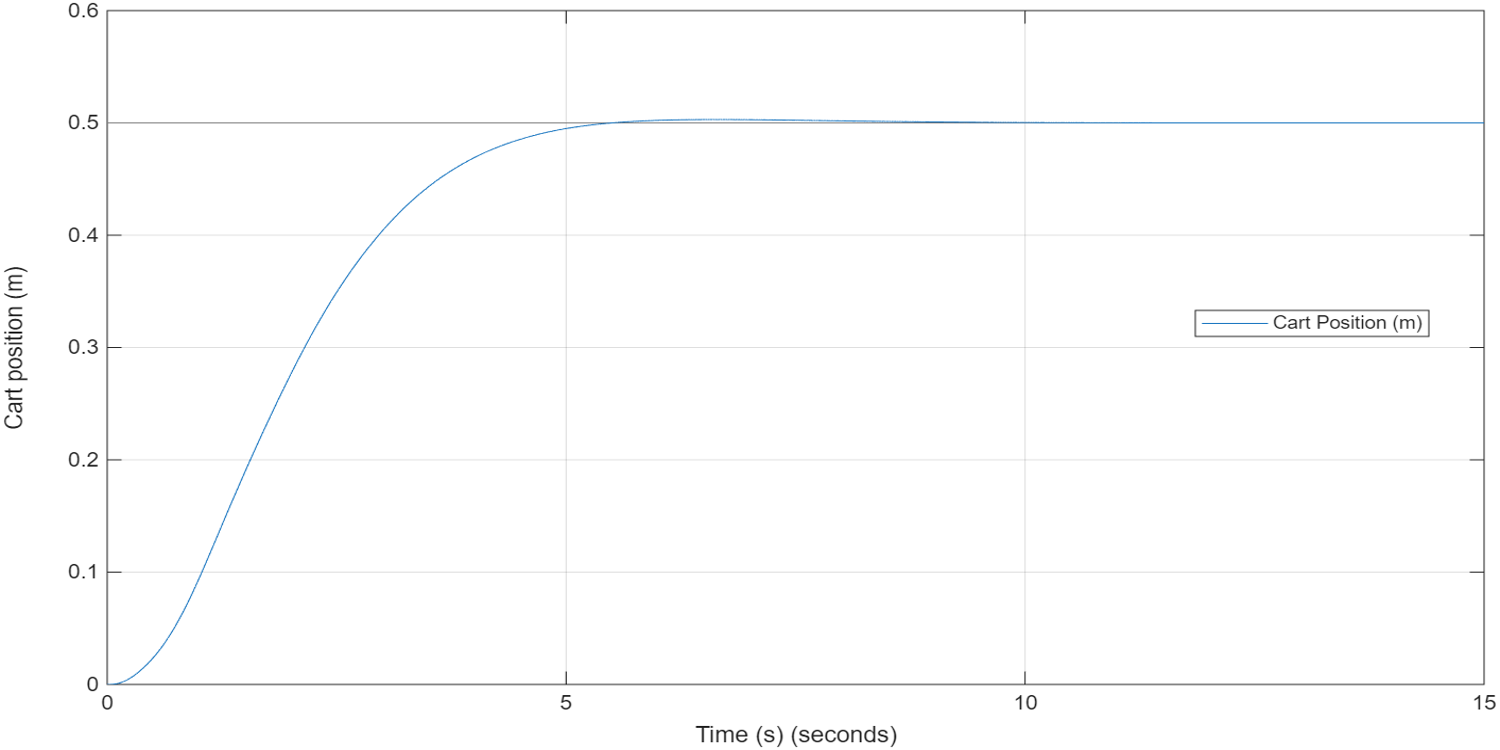
\includegraphics[width=\columnwidth]{Figuras/grafica_carrito_s.png}
\caption{Simulated cart position $p(t)$ using the LQR
controller for a \SI{0.5}{m} step reference.}
\label{fig:lqr_sim_pos}
\end{figure}

\begin{figure}[H]
\centering
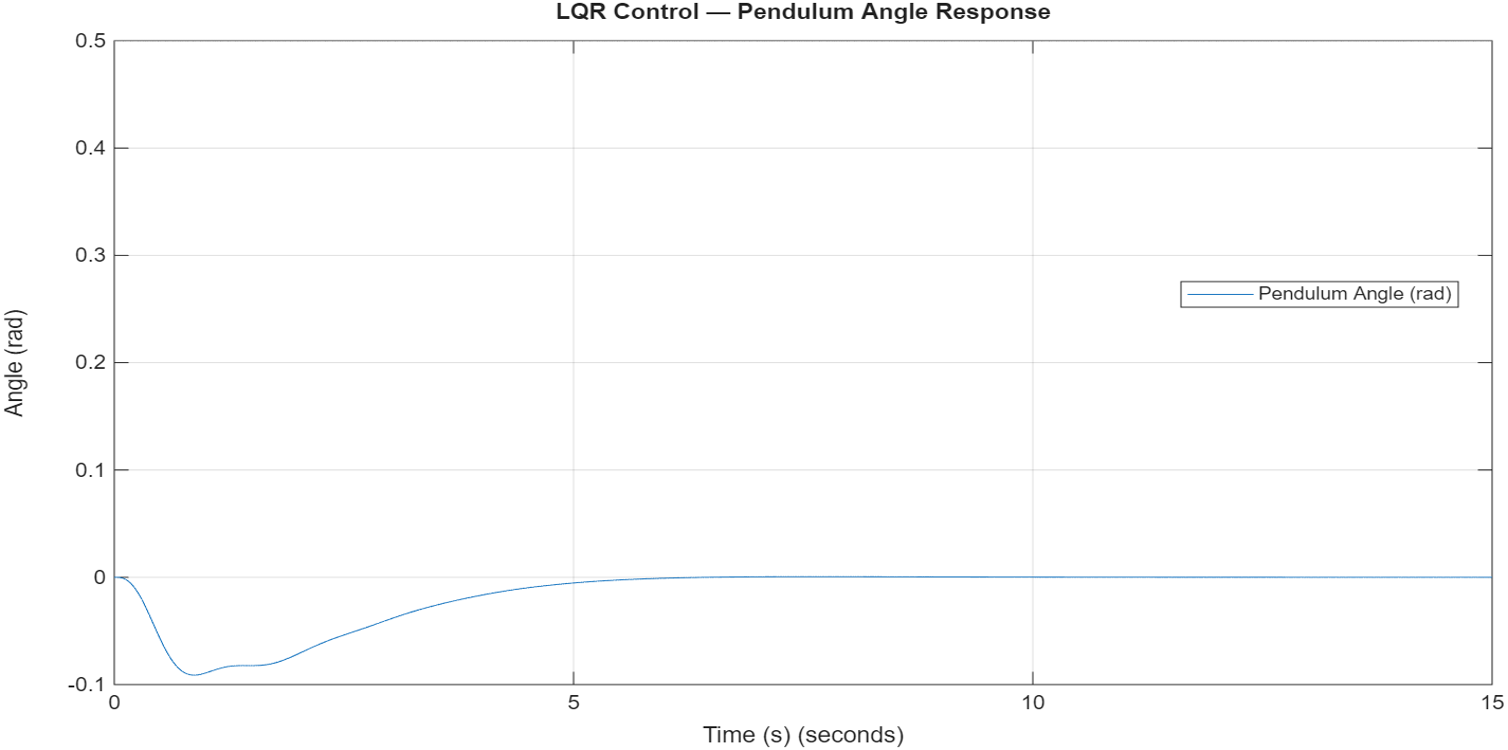
\includegraphics[width=\columnwidth]{Figuras/grafica_angle_s.png}
\caption{Simulated pendulum angle $\theta(t)$ using the LQR
controller for a \SI{0.5}{m} step reference.}
\label{fig:lqr_sim_ang}
\end{figure}

\subsubsection{Experimental Results}

The controller was subsequently implemented on the physical
plant. The measured performance metrics were:

\begin{itemize}
    \item Settling time: $t_s = 5.25$ s
    \item Overshoot: $M_p = 0\%$
    \item Zero steady-state error
\end{itemize}

The experimental cart position response is shown in
Fig.~\ref{fig:lqr_exp_pos}, and the pendulum angle response
in Fig.~\ref{fig:lqr_exp_ang}.

\begin{figure}[H]
\centering
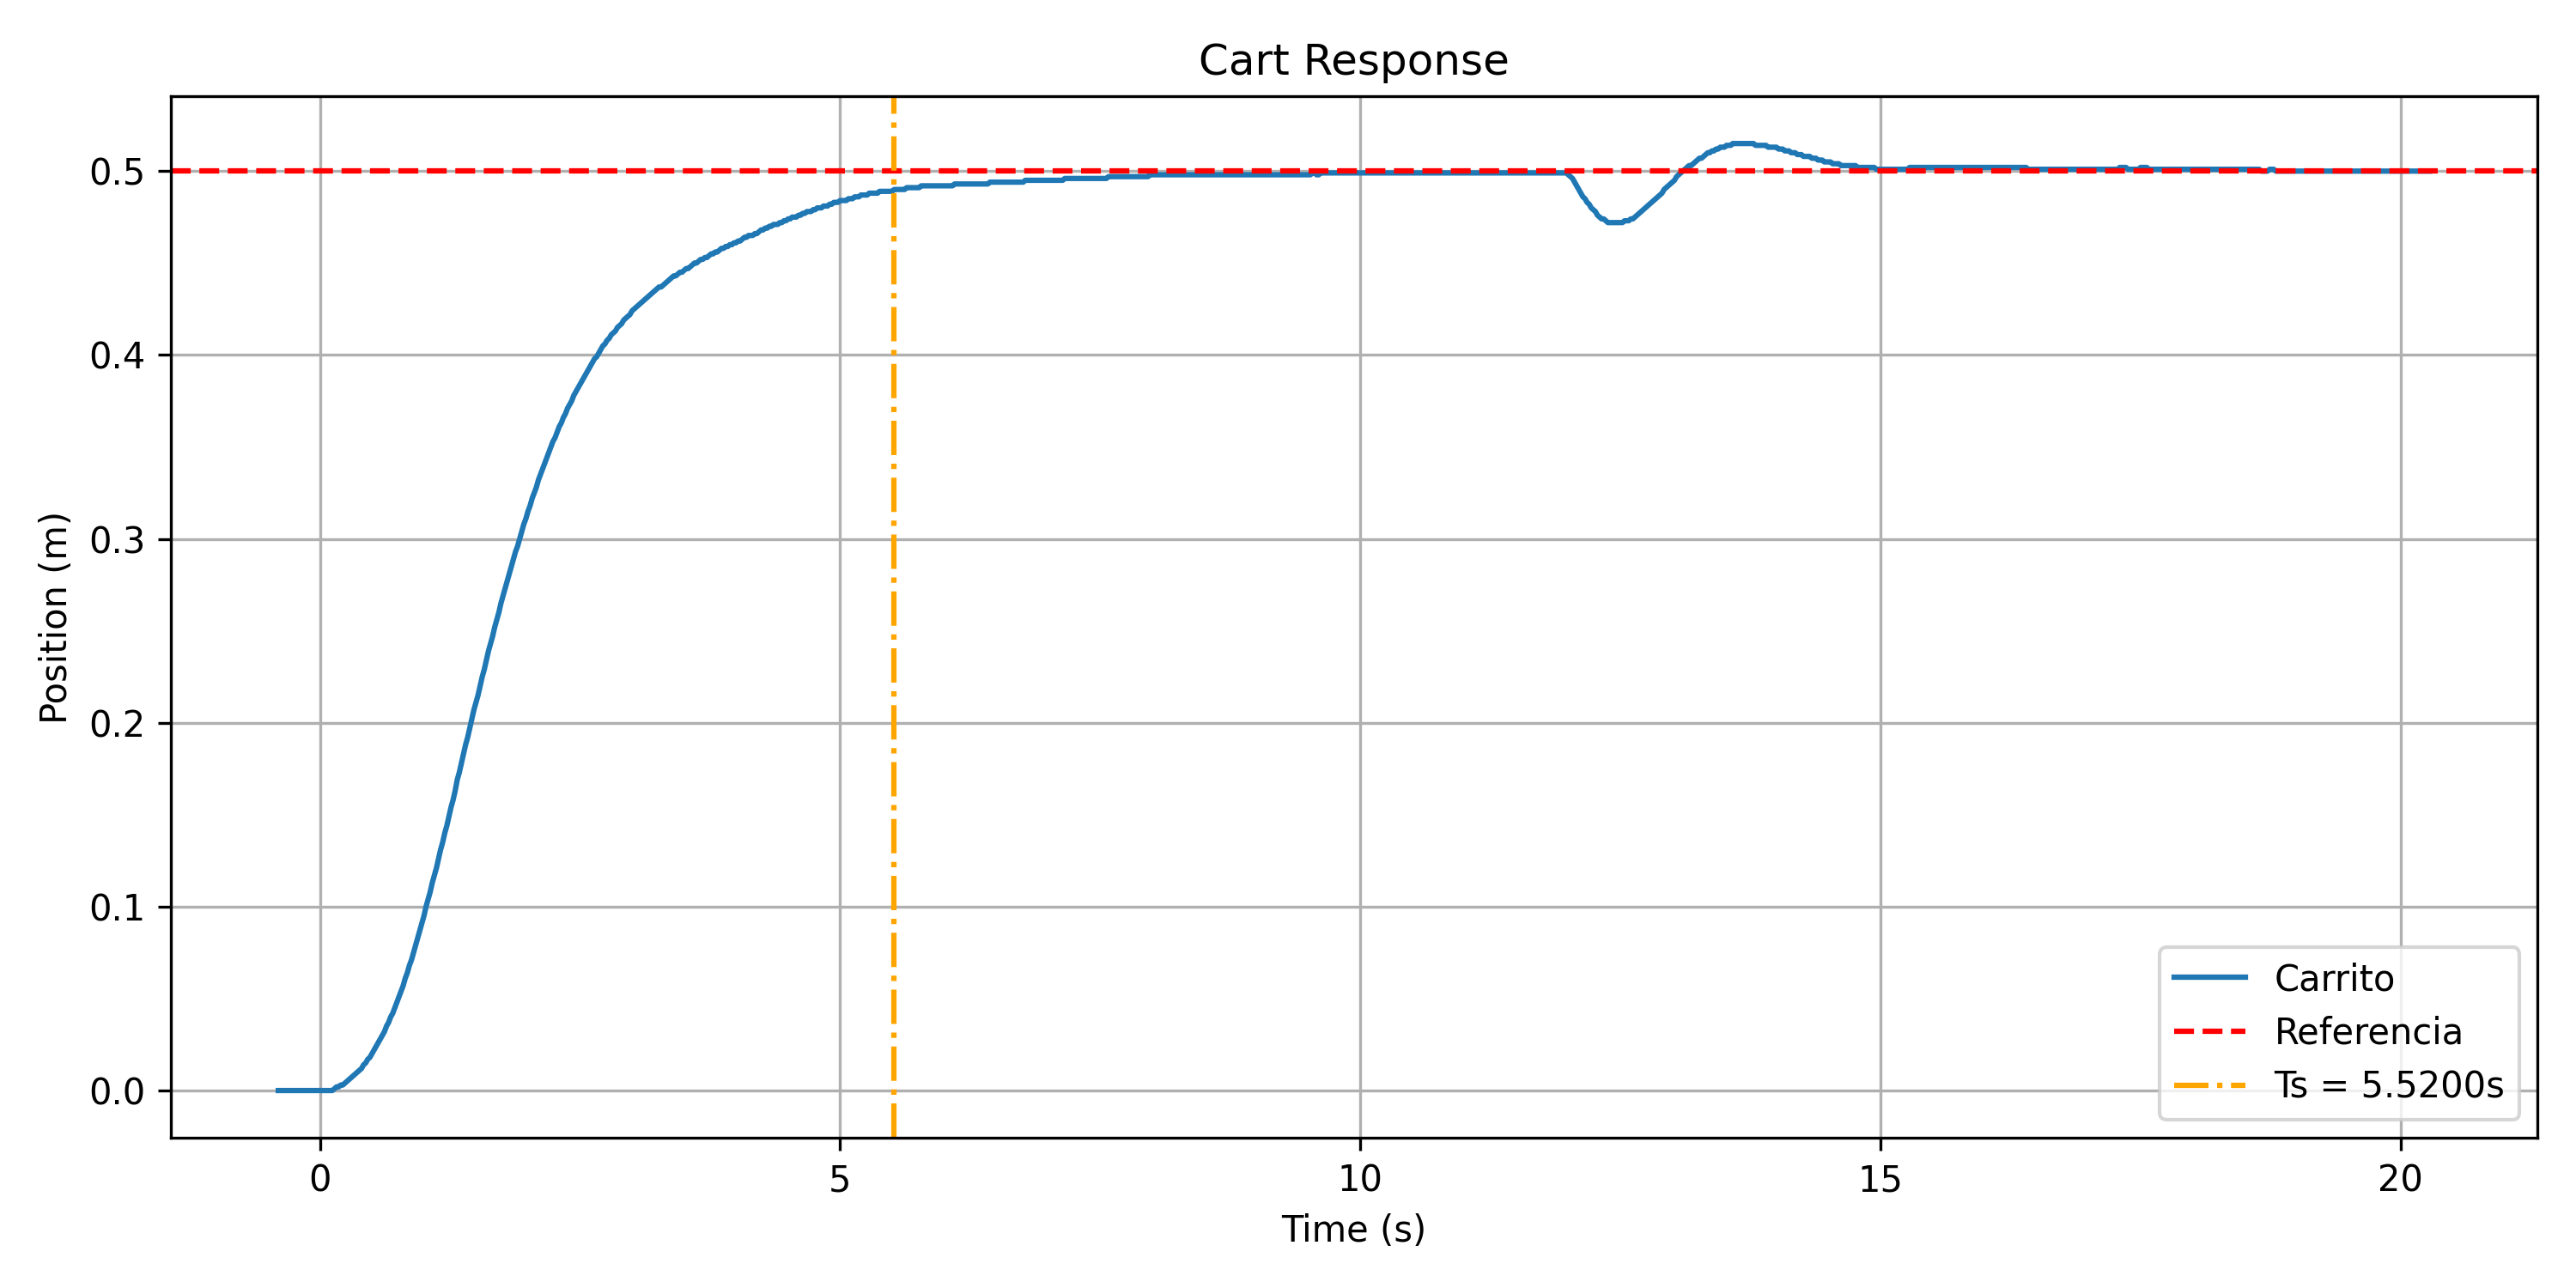
\includegraphics[width=\columnwidth]{Figuras/grafica_carrito.png}
\caption{Experimental cart position $p(t)$ using the LQR
controller for a \SI{0.5}{m} step reference.}
\label{fig:lqr_exp_pos}
\end{figure}

\begin{figure}[H]
\centering
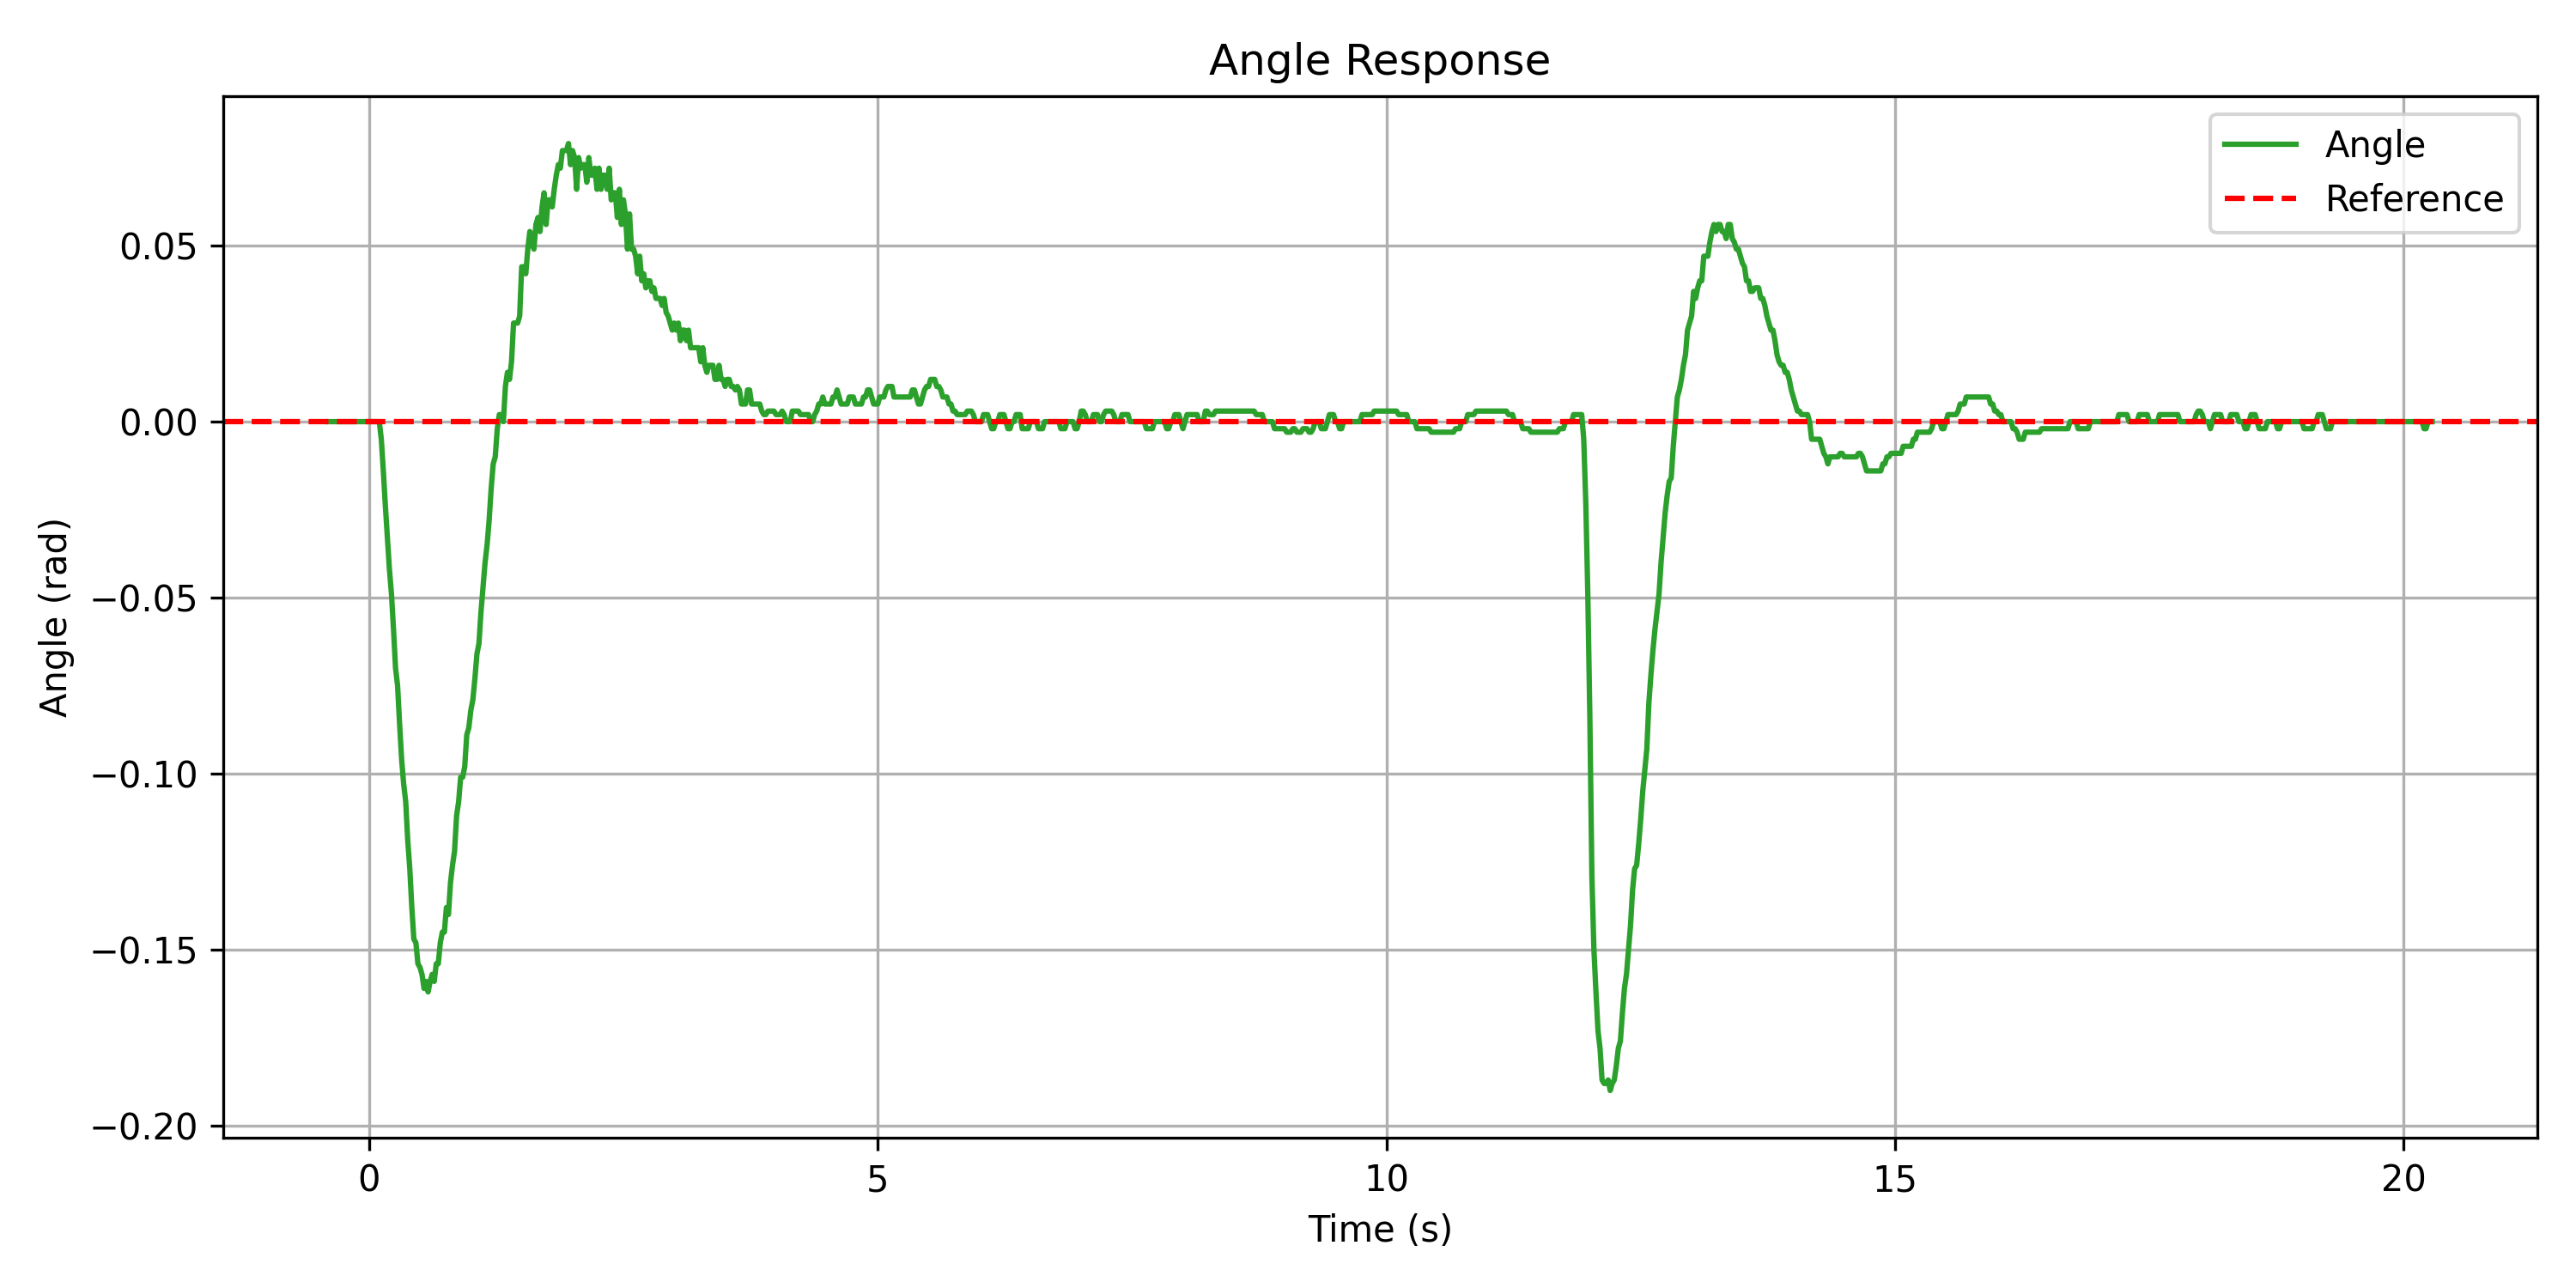
\includegraphics[width=\columnwidth]{Figuras/grafica_angulo.png}
\caption{Experimental pendulum angle $\theta(t)$ using the
LQR controller for a \SI{0.5}{m} step reference.}
\label{fig:lqr_exp_ang}
\end{figure}

The experimental results are consistent with the simulated
response, with a moderate increase in settling time
attributable to nonlinear effects not captured by the
identified linear model, such as friction, motor dead-zone,
and actuator saturation. The absence of overshoot in the
experimental response suggests that the physical damping
exceeds that of the linearized model.

\subsection{Controller Comparison}

Table III summarizes the performance metrics of both
controllers.

\begin{table}[H]
\centering
\caption{Controller Performance Comparison}
\begin{tabular}{lcccc}
\toprule
Controller & Condition & $t_s$ (s) & OS (\%) & $e_{ss}$ \\
\midrule
Pole Placement & Simulation   & -- & -- & -- \\
               & Experimental & --    & --    & -- \\
\midrule
LQR            & Simulation   & 4.701 & 0.601 & 0 \\
               & Experimental & 5.25  & 0     & 0 \\
\bottomrule
\end{tabular}
\label{tab:comp}
\end{table}


\section{Discussion}


\section{Conclusions}


\begin{thebibliography}{99}

\bibitem{ogata}
K. Ogata,
\textit{Modern Control Engineering},
5th ed.
Prentice Hall, 2010.

\bibitem{ljung}
L. Ljung,
\textit{System Identification: Theory for the User},
2nd ed.
Prentice Hall, 1999.

\bibitem{anderson}
B. D. O. Anderson and J. B. Moore,
\textit{Optimal Control: Linear Quadratic Methods}.
Prentice Hall, 1990.

\bibitem{franklin}
G. F. Franklin, J. D. Powell, and M. L. Emami-Naeini,
\textit{Feedback Control of Dynamic Systems},
4th ed.
Prentice Hall, 1998.

\bibitem{mathworks}
MathWorks,
``System Identification Toolbox Documentation,'' Available:
\url{https://www.mathworks.com/help/ident/}

\end{thebibliography}

\end{document}